\section{Introduction and Overview}
Introduce the task at hand.


In this chapter the background and motivation for this paper is presented. The historical development of batteries are presented shortly and former work are presented. 

 
\subsection{Motivation}
%*) Why batteries are important (i.e. cell phones, cars). 

The motivation for this work originates from the rapidly increasing demand for better batteries, both for vehicular and stationary applications. Better batteries mean better products, with longer life, lower cost, and adequate energy storage options. Due to the complexity of the chemical processes involved, it is of high importance to be able to develop predictive modeling methods to improve the search for better compositions and performances






\subsection{History and evolution of batteries}
Never been a more needing market for batteries. Tremendous amount of resources are used on an international level to produce batteries with higher capacity, voltage and energy density. The evolution of batteries started in Italy in the year 1800 by Alessandro Volta (1745 - 1827) that made the first known battery\cite{volta1800electricity}. His invention was the voltaic pile, zinc and copper plates stacked on top of each other with sheets of  bine-soaked cardboard between each plate. The revolutionary property of the voltaic pile was that it could produce a stable current over some time, and not just short sparks of electricity. This invention was the foundation of todays modern battery. \ref{fig:voltaicpile}


\begin{figure}[H]
    \centering
    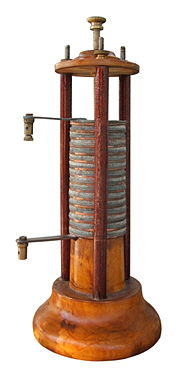
\includegraphics[width=0.2\textwidth]{Pila_di_Volta.jpg}
    \caption{A voltaic pile, the first battery \cite{wiki:voltaicpile} }
    \label{fig:voltaicpile}
\end{figure}

It took almost $40$ years, 1836, before the British inventor John Frederic Daniell Voltas continuation with the discovery of the Daniell cell \cite{daniell1836xi}. The Daniell cell is constructed with to half cells, one with a zinc electrode in a zinc sulfate dissolution, and another copper electrode in a copper sulfate solution. These half cells are connected by a salt bridge. This cell could give a voltage of $\SI{1.1}{V}$ through the reaction shown below, \ref{eq:Daniell}. 


\begin{align}\label{eq:Daniell}
\ce{Zn_{(s)}} + \ce{Cu^{2+}_{(aq)}} \rightarrow \ce{Zn^2+_{(aq)}} + \ce{Cu_{(s)}} 
\end{align}

\begin{figure}[H]
    \centering
    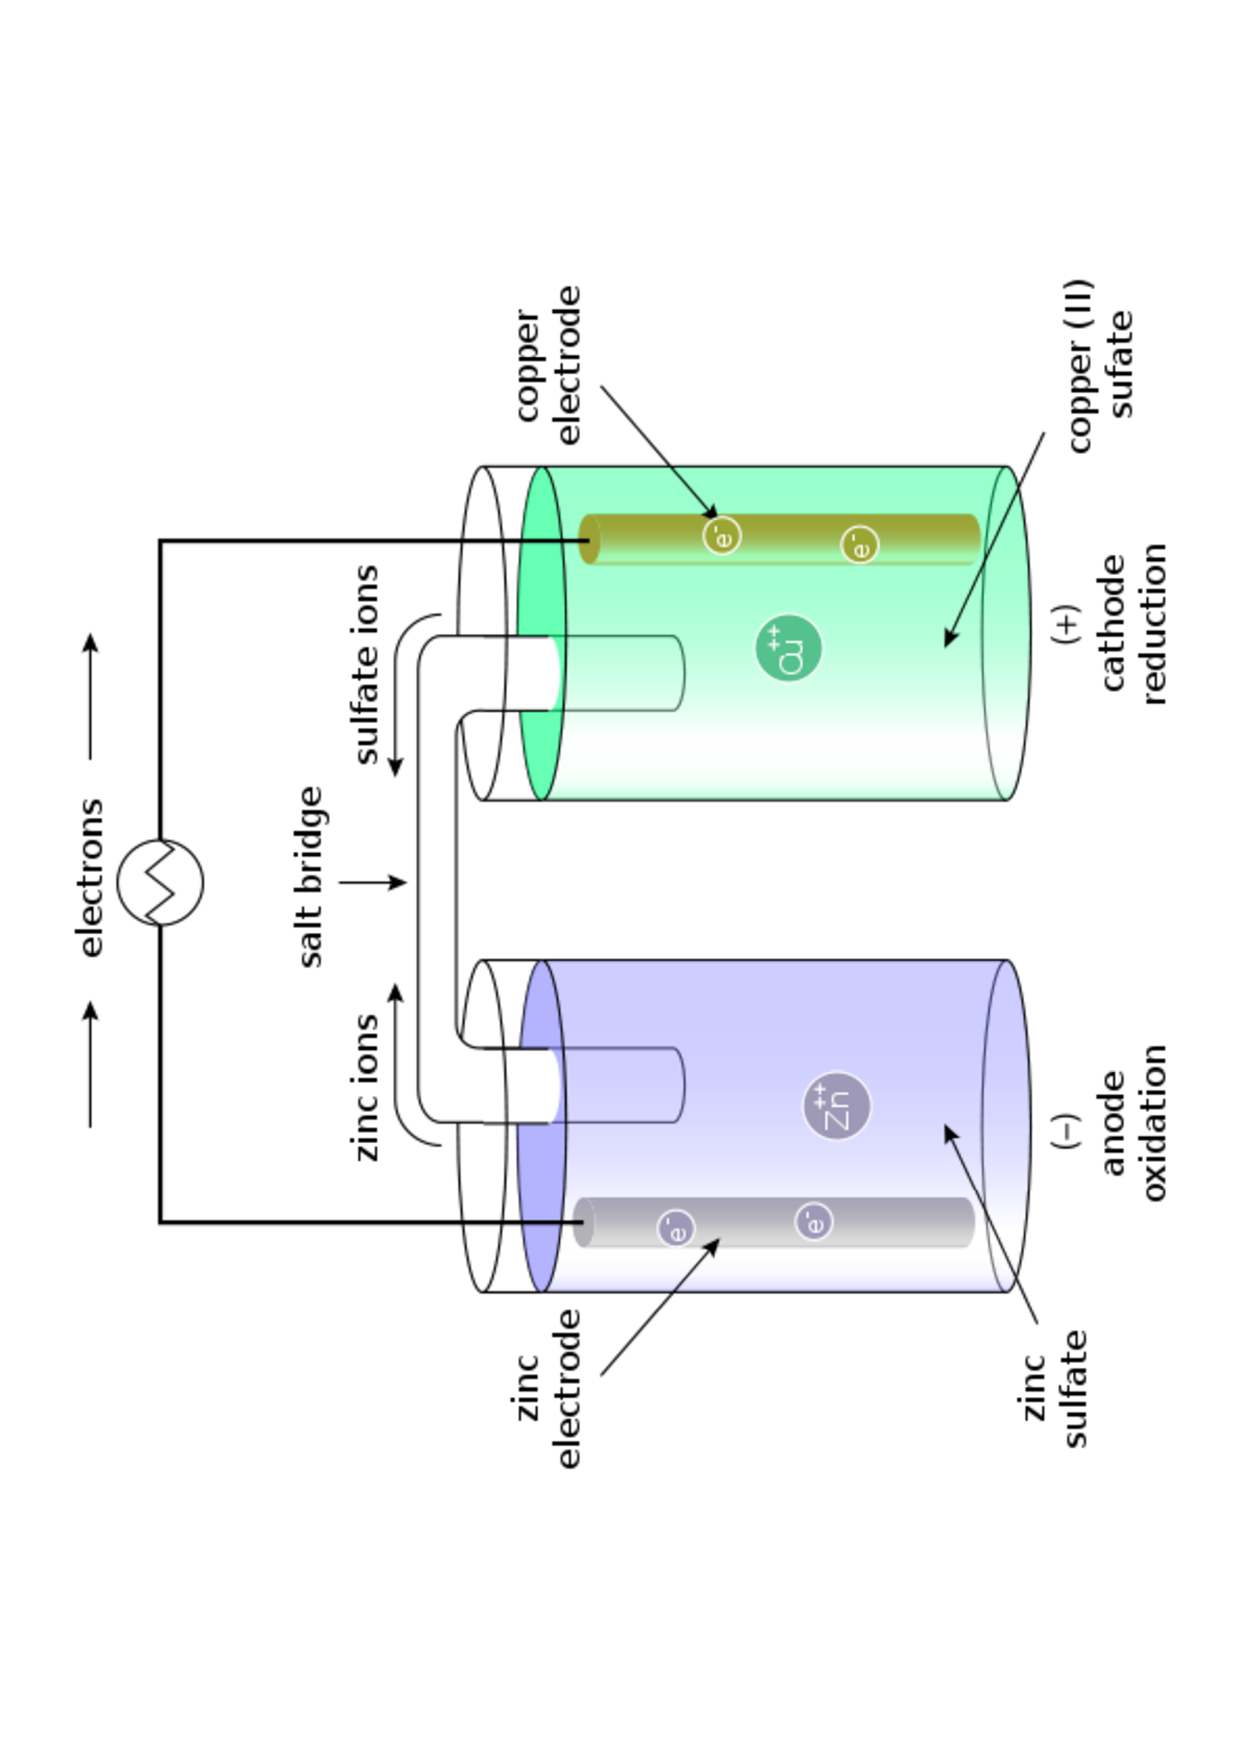
\includegraphics[angle=270,width=0.8\textwidth]{600px-Galvanic_cell_labeled.pdf}
    \caption{A draft of a Daniell cell. The anode is a piece of zinc and the cathode a piece of copper. The salt bridge transports ions between the solutions and the electrons moves through an external circuit. Figure recovered from \cite{wiki:Daniellcell} }
    \label{fig:DaniellCell}
\end{figure}


In 1859 constructed the french physicist Gaston Planté the first led-acid battery. The battery could be charged by applying an external opposite potential, and it was the first secondary battery every made. Planté rolled two led plates into a spiral, separated by rubber stripps, so that the plates would not touch. The lead-acid battery was special due to the electrolyte being a active part of the chemical reaction in the battery. The electrodes in the battery were led anode, and led$(IV)$oxide cathode, immerse din sulfuric acid. The overall reaction is shown beneath: \ref{eq:Plante}. Both the anode and the cathode are made into led(II)sulfate during discharged. The charge is depleted in the electrolyte when the battery is completely discharged(The sulfuric acid has a lower density). Charging changes the electrolyte back into concentrated sulfuric acid. 

\begin{align}\label{eq:Plante}
\ce{PbO_{2(s)}} + \ce{Pb_{(s)}} \ce{2H_2SO_{4(s)}} \rightarrow \ce{2PbSO_{4(s)}} +\ce{2H_2O_{(l)}}
\end{align}

The open circuit voltage$(V_{OC})$ for a led-acid battery are approximately $\SI{2}{V}$. It is custom to attach these batteries in series to attain a higher voltage, typical $6$ or $\SI{12}{V}$. These batteries have a shelf- and cycle life. Normally more then $10$ years or 1000-2000 cycles. They are still in use in modern cars. Led-acid batteries have a relative low \textit{specific energy}, which means that the current is low compared to its weight, they are also renowned for their high environmental impact. Therefor, one of the many goals of battery producers are to replace led-acid batteries with better alternatives.  

Nickel-cadmium$(\ce{NiCd})$ batteries was first described by the swede Waldemar Jungner in 1899 \cite{daniel2012handbook}. These batteries rose fast in popularity due to their high energy density, low weight, long shelf life, and their relative fast recharge. Typically they yield a voltage of $\SI{1.4}{V}$. The cathode is made of Nickel oxide hydroxide, and the anode is made of metallic cadmium, while the alkaline electrolyte is a basic solution of potassium hydroxide. The Specific energy of a typical Nickel-cadmium is $40-60\text{ }\si{W h/kg}$. Equation \ref{eq:NiCdb} shows the overall reaction of such a battery.

\begin{align}\label{eq:NiCdb}
\ce{2NiOOH} + \ce{Cd} + \ce{2H_2O} \rightarrow \ce{2Ni(OH)_2} + \ce{Cd(OH)_2}
\end{align}

Nickel-metal hydride $(\ce{NiMH})$  batteries was first commercialized in the 1980's and had several similarities with the $\ce{NiCd}$ batteries. The main difference is the anode where in  $\ce{NiCd}$ batteries it is  $\ce{Cd}$, while in $\ce{NiMH}$ it is replaced by an alloy that makes metal hydrides (\ce{MH}). $\ce{NiMH}$ batteries has the same electrolyte as $\ce{NiCd}$ batteries, a watery solution of potassium hydroxide. The nominal cell voltage of such a battery is typically around $\SI{1.2}{V}$ and the Specific energy is $60-120\text{ } \si{Wh/kg}$. Equation \ref{eq:NiMH} shows the overall reaction of a $\ce{NiMH}$ battery.

\begin{align}\label{eq:NiMH}
\ce{Ni(OH)_2} + \ce{M} \rightarrow \ce{NiO(OH)} + \ce{MH}
\end{align}

A primary cell is a battery that can not be recharged after use. These batteries are normally used in remote controls, flashlights, and other small household appliances. Alkaline manganese batteries, or just alkaline batteries, are one of the most common primary cells in modern society. Anodes of zinc, cathodes of manganese oxide and a electrolyte of potassium hydroxide, from where it gets its nickname. A typical alkaline battery delivers a nominal cell voltage of $\SI{1.5}{V}$. The overall reaction for a alkaline battery is shown below \ref{eq:alkalineb}.

\begin{align}\label{eq:alkalineb}
\ce{Zn} + \ce{2MnO} +\ce{H_2O} \rightarrow \ce{ZnO} + \ce{2MnO(OH)}
\end{align}

%---------------------------------------------------------------
\subsection{Lithium based batteries}

In 1975 discovered Micheal Stanley Whittingham the intercalation electrodes for lithium and other alkaline metals \cite{whittingham1975lithium}. This led to the first lithium batteries with titanium disulfide$(\ce{TiS_2})$ as the cathode and metallic lithium as the anode. $\ce{TiS_2}$ -structure is divided into layers and lithium-ions can easily move in and out of the structure without significant changes in the structure, which makes the reaction reversible. Figure \ref{fig:MPTiS2} shows the layered structure of $\ce{TiS_2}$. During discharge of the battery, lithium-ions leave the anode of metallic lithium and moves through the electrolyte and into the empty octahedral position in the $\ce{TiS_2}$-structure, while titanium(IV) reduces to titanium(III). While applying an over-potential to the material, or charging, the lithium-ions moves out of the $\ce{TiS_2}$-structure and titanium oxides back to titanium(IV) again. This discovery was the start of a major research investment in cathode materials of sulfite and other chalcogens in the 70-80's. 


\begin{figure}[H]
    \centering
    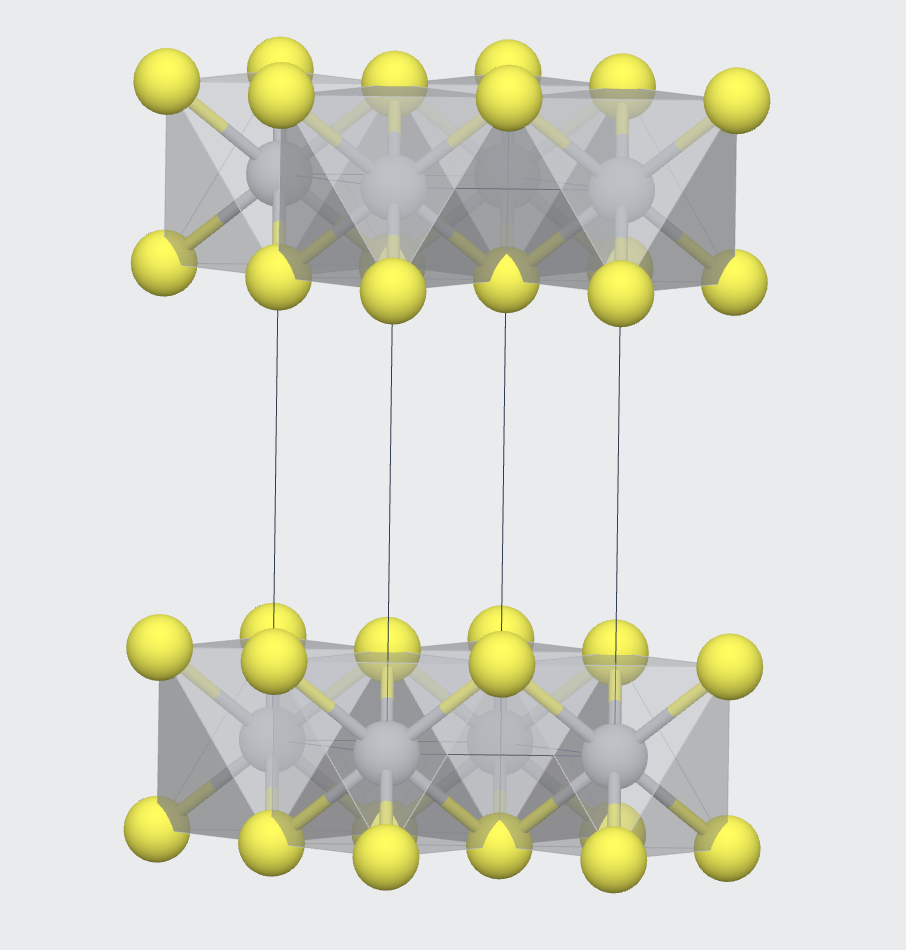
\includegraphics[width=0.4\textwidth]{TiS2.png}
    \caption{The two-dimensional trigonal omega-like structure of $\ce{TiS_2}$. Observing from a slight angle along the b-axis. The titanium in \textcolor{gray}{grey}, are occupying the octahedral holes of sulfur, in \textcolor{yellow}{\textbf{yellow}}. Lithium-ions would intercalate into the space between the $\ce{TiS_2}$ layers. Figure attained from materialspoject \cite{materialsproject:TiS2}.}
    \label{fig:MPTiS2}
\end{figure}

It is of the utmost importans that the Lithium-ions in a lithium battery can easily be intercalated and extracted (\myworries{Can I phrase it like this?}) in a reversible manor, and such layered structures are especially good for this purpose. In 1980 introduced John B. Goodenough $\ce{LiCoO_2}$ as the cathode material for lithium batteries, a material that gave a $V_{OC}$ of $4-5\text{ } \si{V}$, which opened up many possibilities to alternate the negative electrodes, and earned him, M. Stanley Whittingham and Akira Yoshino the Nobel Prize in Chemistry. Goodenough and colleagues  found a current density of up to $\SI{4}{mAcm^{-2}}$ \cite{mizushima1980lixcoo2} \cite{goodenough1980solid}. Even though the properties where exceptionally good at the time, the batteries were still not commercialized due to metallic lithium being unstable, and deemed to be an unsafe anode. This was due to dendrites growing out of the anode that short circuited the battery. 

In $1990$ introduces Sony lithium batteries on the commercial market. They had exchanged the metallic lithium anode for graphite which reduced the growth of dendrites on the anode. The electrolyte was a organic solvent with a lithium salt. A lithium-ion battery refers to a battery where lithium intercalates in both electrode materials, both the cathode and the anode. While lithium batteries has a anode of metallic lithium. This nomenclature is transferable to other type of batteries like, magnesium/magnesium-ion batteries. 

Figure \ref{fig:LiCoO2} shows a draft of a lithium-ion battery with $\ce{LiCoO_2}$ as the cathode and graphite as the anode. During discharged the lithium-ions moves from the anode, through the electrolyte and separator to the cathode. The electron moves from the anode to the cathode through a separat circuit, where the electrical energy can be extracted. The overall reaction is shown in equation: \ref{eq:LiB}

\begin{figure}[H]
    \centering
    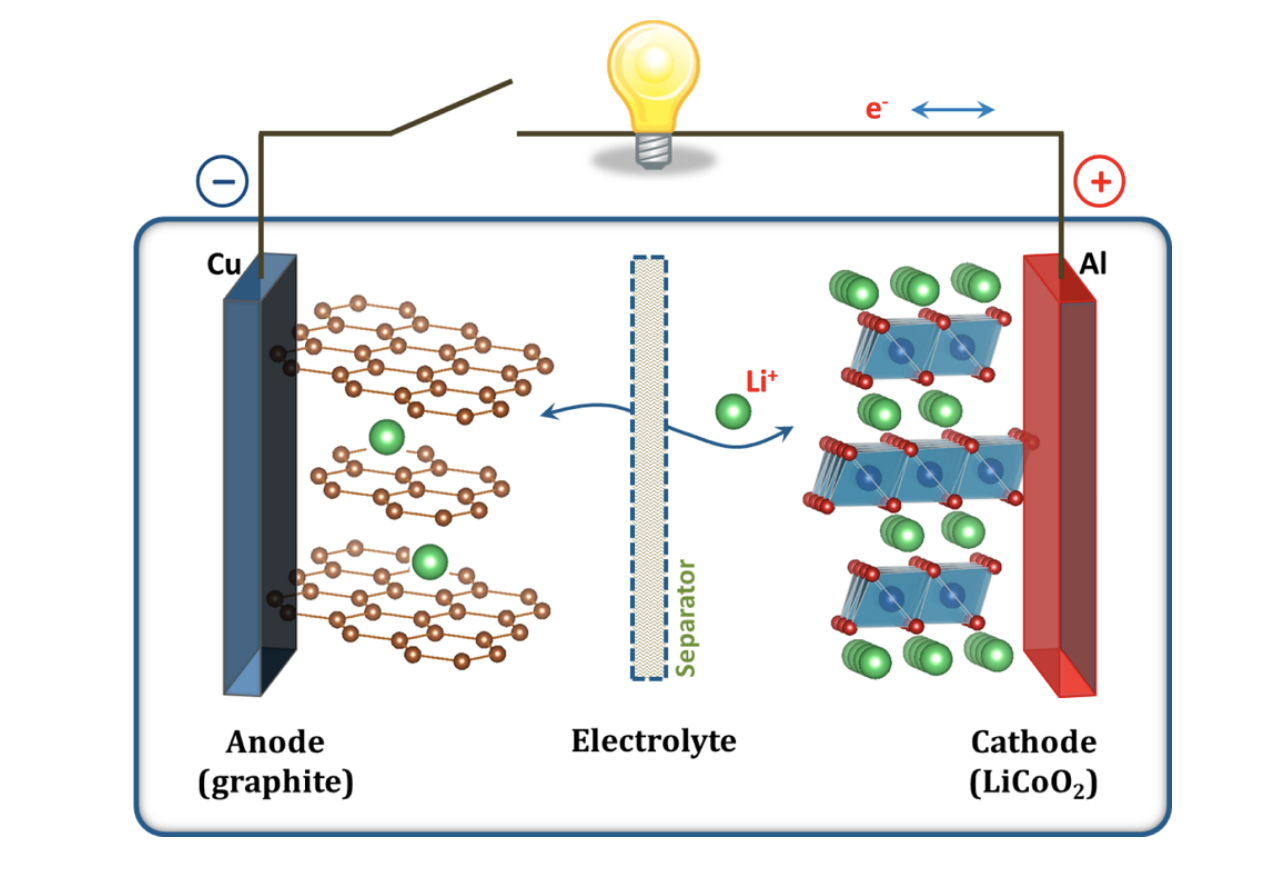
\includegraphics[width=0.4\textwidth]{Li-ion_inter.png}
    \caption{Schematic illustration of the first Li-ion battery $\ce{LiCoO_2/Li^+}$ electrolyte/graphite), Figure acquired from  \cite{goodenough2013li}.}
    \label{fig:LiCoO2}
\end{figure}

\begin{align}\label{eq:LiB}
\ce{LiCoO_2} + \ce{C_6} \rightarrow \ce{Li_{1-x}CoO_2} + \ce{Li_xC_6}
\end{align}

The cathode materials used in lithium-ion batteries have evolved since the 1990 until today. Normal cathode materials today are $\ce{LiMn_2O_4}$ and $\ce{LiFePO_4}$. Neither of the two has a layered structure as in the $\ce{SO_2}$ structure, but $\ce{LiMn_2O_4}$ is a good ionic conductor due to the structure having canals in all three dimensions where lithium can be transported, see \ref{fig:LiMnO2}. While $\ce{LiFePO_4}$ has a lower ionic conductivity, due to it only having  canals in one dimension, see figure \ref{fig:LiFePO4}. It is still a popular material due to its high cycle life. There still exist layered structures that are in use in batteries.


\begin{figure}[H]
    \centering
    \begin{subfigure}{0.30\textwidth}
        \centering
        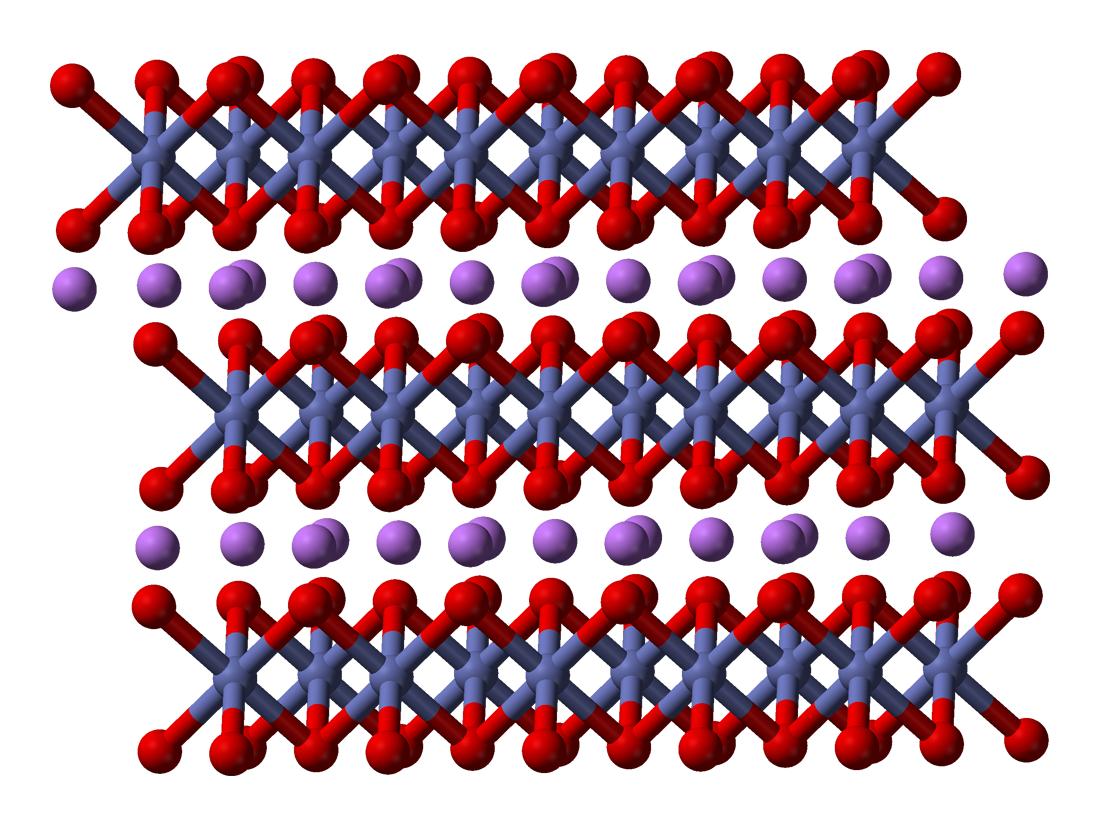
\includegraphics[width=\linewidth]{Lithium-cobalt-oxide-3D-balls.png}
        \label{fig:LiCoO2_pic}
        \caption{}
    \end{subfigure}%
    ~ 
    \begin{subfigure}{0.36\textwidth}
        \centering
        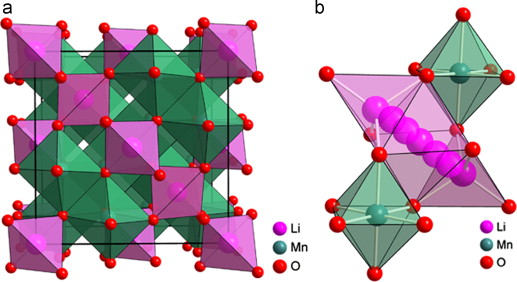
\includegraphics[width=\linewidth]{a-Crystalline-structure-of-spinel-LiMn2O4-and-b-its-corresponding-lithium-diffusion}
         \label{fig:LiMnO2}
        \caption{}
    \end{subfigure}
    ~ 
        \begin{subfigure}{0.30\textwidth}
        \centering
        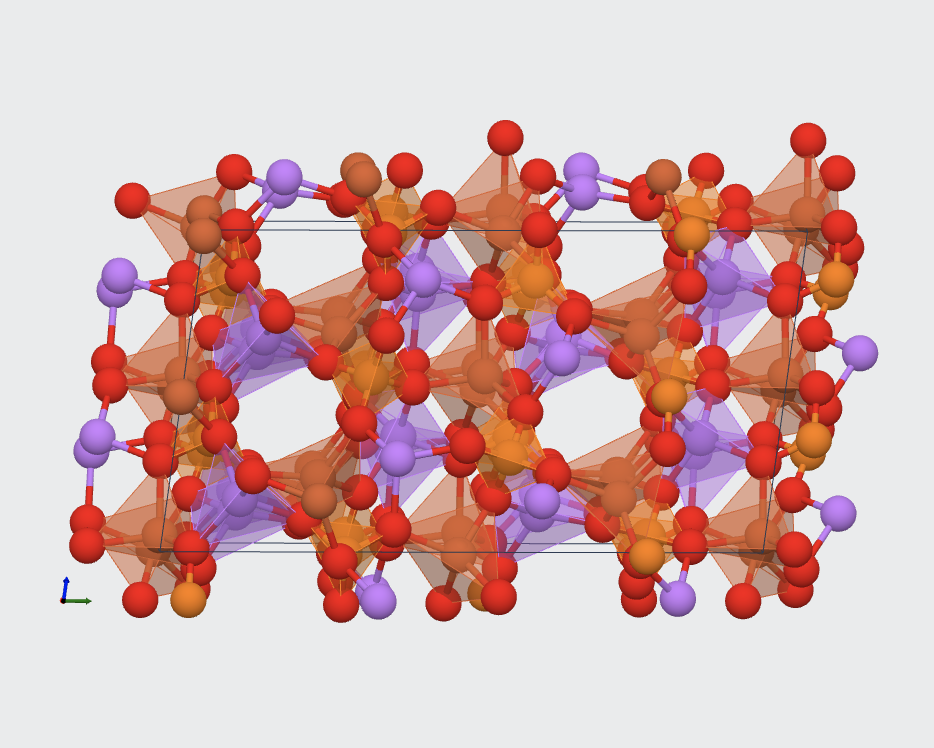
\includegraphics[width=\linewidth]{LiFePO4.png}
        \caption{}
        \label{fig:LiFePO4}
    \end{subfigure}
	\caption{Crystal structures of a)$\ce{LiCoO_2}$\cite{wiki:LiCoO2} b) $\ce{LiMn_2O_4}$\cite{zhang2013understanding}, c) $\ce{LiFePO_4}$\cite{materialsproject:LiFePO4}. The layers in $a)$, the canals in $b)$ and $c)$ are illustrated.}
	\label{fig:Li_a-c}
\end{figure}

The most used anode materials for lithium-ion batteries are graphite and other forms of carbon based materials. Graphite has a high energy density, making the cathode material the limiting factor for energy density of Lithium-ion batteries. To improve the cathode material is therefore high in priority. 

There is an ongoing search for candidates for solid-state electrolytes, due to energy density and safety being the main factors that govern the development of the rechargeable battery technology \cite{guzik2019lightweight}. This is not just limited to Lithium-ion batteries other active elements as Na and Mg are also being explored. Solid-state electrolytes would enable stable and reliable operation of all-solid-state Li-, Na-, and Mg-based batteries. Special focus is given to lightweight complex metal hydrides, due to them showing high ionic conductivity, and in some cases electrochemical properties that enable battery reversibility. \myworries{move this to later.}


%----------------------------------------------------------------------
\subsection{Magnesium batteries}
The abundance of magnesium in the earth's crust, combined with its low atomic weight, low cost, and electrochemically active nature, makes magnesium a great candidate for battery applications. It can serve as a potential negative electrode with its electrochemical potential of $\SI{-2.37}{V}$. It is environmentally friendly due to its by-products being safely excreted through urin.  

renowned as a primary battery

secondary battery rising!
The first prototype of a Magnesium secondary cell was produced 


%----------------------------------------------------------------------
\subsection{Earlier work}



%----------------------------------------------------------------------
\subsection{Scope of the thesis}
%Clarify what you want to cover. 
Write more about: PV, wind, solar -> storage.

"At what cost can one charge stationary secondary batteries with solar/wind power efficiently, and provide a centralized energy storage? For what shelf and cycle life? with how rapid a respons  a power outage or fluctuation in the grid. And with how large a capacity, at a competitive cost? " \myworries{where?}


%Why batteries are important(Cars how many in how long? )
Batteries are vastly complex and much efforts have been devoted to the development of these. Yet, with all the efforts put in to electrochemical cells, there are still a never ending chase for batteries that can push the limits of their properties even further. The demand for better batteries are growing faster then ever. The global electric car fleet, for instance, exceeding 5.1 milion\cite{international2018global}, almost doubling the number of new electric car registrations in the last year. And if we follow the policies of the EV30@30 Scenario which aims to reach a $30\%$ market share for EVs in all models except two wheelers by 2030, due to one quarter of global greenhouse gas(GHG) emissions comes from this sector. The EV sales per year are then predicted to be more then 43 milion, and the stock numbering more than 250 milion.  

This work proposes a methodology to predict these properties accurately without the need of big scale simulations, or computer heavy calculations. Using state of the art machine learning, and base properties of all ready existing databases, we propose a set of predictors to see if we can predict the properties of new, undiscovered electrodes, or even new properties in already well known electrodes.

%*) What are the most important properties that todays batteries should improved (i.e. higher capacities, longer life times (durability) etc.)
Some of the most important cell properties are; voltage, energy density, specific energy or capacity, flammability, available cell constructions, operating temperature range, shelf life or self discharge, low cost, and worldwide consumer distribution. Most of these properties are to an extent dictated by battery chemistry. And it is of the general publics interest to improve several of these characteristics, both for once pleasure (i.e. several more hours to play candy crush), and the peoples general safety (i.e. electric car crashes, and Samsung phones). In this work we will focus on the  base properties; voltage, energy density, specific energy, and the physical stability of the materials. No real battery fulfills all of these requirements. And most real batteries underperforms  We therefore leave the safety issues to the experimentalists.


%*) What is a typical procedure for designing a new battery ( a general discussion from the experimental and theoretical point of view)
The idea behind the designe of a battery is fairly simple, due to their similar procedure to create electricity. Two of the most important parts are the Anode and the Cathode. A cell produces electricity when placed into a medium that has conductive properties, namely the electrolyte.


%*) Focus on the theoretical part. What theoretical techniques are used today for the design of new batteries (i.e. DFT calculations,  molecular dynamics simulations etc). Provide some references.

Today some of the main methods for theoretical advances in battery science are density functional theory (DFT), molecular dynamic simulations and


%*) Make clear if the theoretical results provide useful information during the whole process of building a new battery.

%*) Start discussing that experimental and traditional theoretical approaches are expensive and computationally demanding. From that point on start introducing the need of new theoretical approaches

%*) Make a short introduction to ML. Here you should make clear the following.
%    -- There are already a lot of theoretical and experimental data. Can we use these data for making predictions for unknown materials?
%    -- ML is an approach that  uses past data trying to find relations and correlations between them. Based on them (this is called ML model) the model created can be used for prediction in new unknown materials.
%   -- What are the advantages of the ML approach:
%      a) Is computationally efficient (few minutes/hours to build a model, and no time for making predictions)
%     b) In principle, there is no need to provide any mathematical/physical equations or laws (which maybe are unknown or dont exist) in order to have predictions. The ML model will find them (even though for most of the ML models, these relations can never be undestood by humans....!!!!)
 %    c) In principle you can provide to ML algorithm any information (input). If some of the information  is irrelevant, then the ML algorithm will give zero weight / importance to it. However, providing only a part of the relevant/important information to the ML algorithm will lead to poor predictions.

 %    -- What are the challenges/difficulties of using ML models:
 %   a) Sufficient data (commonly called "examples" by ML experts)
  %  b) Accuracy of the provided data (inputs and output)
  %  c) Usage and if necessary design of the proper descriptors (I mean the inputs that the result depends on)
  %  d) Use of the proper ML technique (i.e. Random forest, SVR, neural networks etc)

%*) Make the statement that usually in real problems of physical chamisty the ML methods can provide good estimations (at best) but not exact predictions. There are several reasons for that, such as, small training examples, accuracy of the training data, not providing all relavant information (descriptors) etc. HOwever, we hope that a good ML model will finally provide us with the most promising materials for a specific application, reducing significantly the number of candidates that the theoretical/experimental studies should focus from this point on. 

%*) Start describing what are the goals of the present work. Give first the battery properties that you consider more important (e.g. capacity). The goal of the work is more or less the following (expand it): can the use as ML descriptors (input) of elemental atomic properties (e.g. atomization energy), and compounds properties (e.g. geometrical features, AP_RDF) can provide reasonable predictions for your goals. 

\subsubsection{Research Question}

How to better batteries?

RQ1: Is there potential for the use machine learning to easy the search for better battery materials?

RQ2: Which ML method would be the most optimal for such a search?

RQ3: What predictors are the most suited for such a task, and which would yield the most efficient training.

RQ4: How does the size of the database affect the results? 

\subsubsection{Approach}

The choice of features examined in this work is inspired by an extensive survey done on similar project especially in the field of Metal Organic Framework(MOFS) done by my supervisors in Crete, and dictated, to some degree by the lack of more data.(REF)

To answer the questions s

In order to evaluate the effect of different features, a prediction approach using principle component analysis was utilized. First we used physical descriptors, geometrical properties of the unit cell, for instance. This because it was greatly efficient in similar studies(REF) on MOFS, and is straightforward. 
Other descriptors are needed, and the void fraction seemed like the next obvious one, that is both geometrical and easy to obtain. Afte

\subsection{Structure of the thesis}

First the most essential concepts from the fields of batteries, machine learning, and work already explored on these two fields conjoined, are introduced. Then the method will be explained before rounding up our results so far before trying to put this all into perspective.